% METODOLOGIA------------------------------------------------------------------

\chapter{MATERIAIS E MÉTODOS}
\label{chap:metodologia}

Neste capítulo será discutida a metodologia empregada para o cumprimento dos objetivos desta pesquisa. Nele, destaca-se a utilização do \textit{GDD} para nortear as atividades de desenvolvimento do jogo; as ferramentas de desenvolvimento de softwares que vêm sendo utilizados pela equipe, focando especificamente nas empregadas para o cumprimento dos objetivos deste trabalho. Também será apresentada a metodologia de processo construção de software empregada, elaborada pela equipe deste projeto.

\section{\textit{Game Design Document (GDD)}}
\label{sec:gdd}

Em geral, as atividades de Game \textit{Design} se situam na criação de um contexto que direciona à todas as outras atividades relacionadas ao desenvolvimento de jogos, como também garantem que a equipe de desenvolvimento compreendeu este contexto e que a execução do trabalho corresponda ao esperado. O cargo do principal responsável da equipe por elaborar o design do jogo corresponde ao Game \textit{Designer} \cite{bib:motta2013}.

De forma prática, o game \textit{design} define: o que determina a jogabilidade, as escolhas que o jogador terá dentro do mundo do jogo e as ramificações que suas escolhas vão ter no resto do jogo. Inclui o que faz o jogador vencer ou perder, como ele vai controlar o jogo, as informações que o jogador deverá receber. Em resumo, o game design descreve cada detalhe de como funcionará a jogabilidade \cite{bib:godoi2013}.

Para tanto, o profissional de game \textit{designer} concebe o documento de game \textit{design}, ou \textit{Game Design Document (GDD)} que, é uma ferramenta textual que descreve todas as características de um jogo, desde informações básicas de premissa, conceitos, passando por personagens e cenários, informações mais detalhadas como projeto de \textit{levels} e até sons \cite{bib:motta2013}. Muitas vezes, esse documento é chamado de ``bíblia"\space do jogo, sendo realmente usado como uma bíblia, uma referência para todos os envolvidos no desenvolvimento do projeto, mantendo todos ligados aos mesmos objetivos.

Já \citeonline{bib:schuytema2008} afirma que ``o documento de game \textit{design} é o coração e a alma de todos os documentos que giram em torno de um game em desenvolvimento". Sendo assim, o autor criou alguns itens que considera essenciais para o \textit{GDD} de um jogo comum (figura \ref{fig:estrutura-gdd}). Dado que, esta estrutura poderá sofrer alterações conforme o tipo de jogo, podendo ter itens adicionados/removidos necessariamente.

\begin{figure}[H]
	\centering
	\caption{Estrutura do Documento de Game \textit{Design}}
	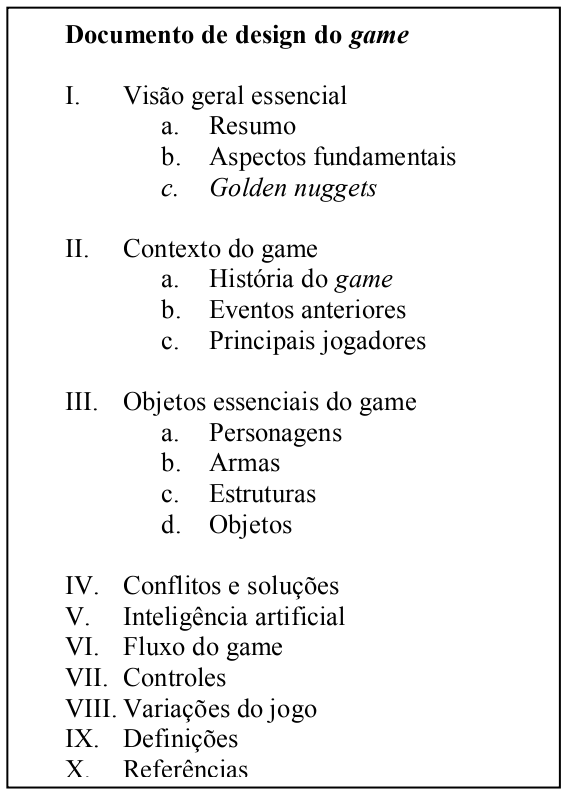
\includegraphics[width=0.6\textwidth]{figuras/estrutura_gdd}
	\label{fig:estrutura-gdd}
	{\fonte{\citeonline{bib:schuytema2008}}}
\end{figure}

De um modo geral, o \textit{GDD} apresenta uma estrutura sistematizada de diversos elementos do jogo: conceito do jogo; mecânicas de jogo; interfaces com usuário; elementos gráficos estáticos, animados e de vídeo; descrição de personagens; enredo e história; sons e música; detalhamento de \textit{levels} (missões) entre outros elementos. Através destes é possível descrever o que um jogo deve ter \cite{bib:motta2013}.

\section{Ferramentas de Desenvolvimento de Jogos}
\label{sec:ferramentas}

Nesta seção são apresentadas as ferramentas de desenvolvimento de jogos que vêm sendo utilizadas para a implementação do projeto ``Araguaia: A Saga de Osvaldão". A seleção das ferramentas deu-se em função da experiência dos membros do LAGE no uso destas, e também o fato da maioria delas possuir licença de software livre, ou uma versão gratuita para estudantes.

\newpage

\begin{itemize}
	\item \textbf{Blender:} É uma ferramenta que permite a criação de vastos conteúdos em \textit{3D}. Oferece funcionalidades completas para modelagem, renderização, animação, escultura digital, pós-produção, criação e visualização de conteúdo \textit{3D} interativo. Originalmente desenvolvido pela empresa \textit{``Not a Number"\space(NaN)}, o \textit{Blender} agora é desenvolvido como ``Software Livre", e o seu código fonte está disponível sobre a licença \textit{GNU GPL}\footnote{https://www.gnu.org/licenses/gpl.html} \cite{bib:blender2018}. Este software foi utilizado para na modelagem da \textit{cutscene} inicial \textit{3D}, descrita na subseção \ref{subsec:cutscene3D}.
	
	\item \textbf{Makehuman:} Usado para a criação dos personagens Osvaldão e menino na \textit{cutscene} inicial, é um programa gratuito e intuitivo de modelagem de personagens humanoides, ele oferece ferramentas que permitem, com um clique do mouse, manipular um modelo de um humano em \textit{3D}, definindo proporções corporais, sexo, roupas, cores e etc \cite{bib:makehuman2018}.
	
	\item \textbf{Inkscape:} É um editor de gráficos vetoriais gratuito, semelhante aos softwares \textit{Adobe Illustrator, Corel Draw} e \textit{Xara X}. O que o torna único é a utilização de \textit{Scalable Vector Graphics (SVG)}, um padrão \textit{W3C} baseado no padrão \textit{XML}, como formato nativo. É utilizado para criação dos personagens (pelos artistas da equipe), elementos do ambiente do jogo e itens de interface gráfica com o usuário \cite{bib:inkscape2016}.
	
	\item \textbf{GIMP:} É uma ferramenta gratuita de manipulação de imagem multiplataforma, que oferece uma variedade de funcionalidades, incluindo retoque de fotos, composição de imagem e construção da mesma. Foi utilizada para tratar (ajustes de inclinação, recortes e etc.) as texturas de modelos tridimensionais para serem utilizadas com o \textit{Blender} no processo de texturização na \textit{cutscene 3D} (descrita na seção \ref{subsec:cutscene3D}) \cite{bib:gimp2018}.
	
	\item \textbf{Unity:} É uma game \textit{engine} (motor de jogos) proprietário criado pela \textit{Unity Technologies}, que é utilizada, juntamente com a linguagem de programação C$\sharp$\footnote{\url{https://docs.microsoft.com/pt-br/dotnet/csharp/programming-guide/}} para integração dos elementos do jogo (cenários, personagens e etc.), dando ``vida"\space e dinamismo aos mesmos (é o software mais importante na criação de um jogo) \cite{bib:unity2018}.
	
\end{itemize}

\section{\textit{Framework} de Desenvolvimento de Jogos Educacionais}
\label{sec:desenvolvimento}

Assim como qualquer produto de software, desenvolver um jogo educativo requer um modelo sistemático de desenvolvimento de software, que possa orientar a equipe para alcançar, da melhor forma possível, os objetivos propostos para o projeto.   

O processo de desenvolvimento do jogo educativo (figura \ref{fig:framework_dev}) foi elaborado com base em duas metodologias. A primeira de \citeonline{bib:guterres2017}, que apresenta um \textit{framework} para apoio à reflexão sobre o processo de produção de objetos de aprendizagem, resultado da triangulação de práticas pertinentes relacionadas ao tema, obtidas a partir de uma revisão de literatura (incluindo uma revisão e um mapeamento sistemático), de observações e de entrevistas com integrantes de nove centros brasileiros de produção de objetos de aprendizagem. A segunda de \citeonline{bib:savi2011}, conhecida como modelo \textit{ADDIE}, sigla para \textit{Analyze, Design, Develop, Implement} e \textit{Evaluate} (Análise, Projeto, Desenvolvimento, Implementação e Avaliação), é um processo genérico, empregado para identificar as necessidades do público-alvo, projetar a solução e avaliar os resultados.

\begin{figure}[H]
	\centering
	\caption{Processo de Desenvolvimento usado no projeto do jogo}
	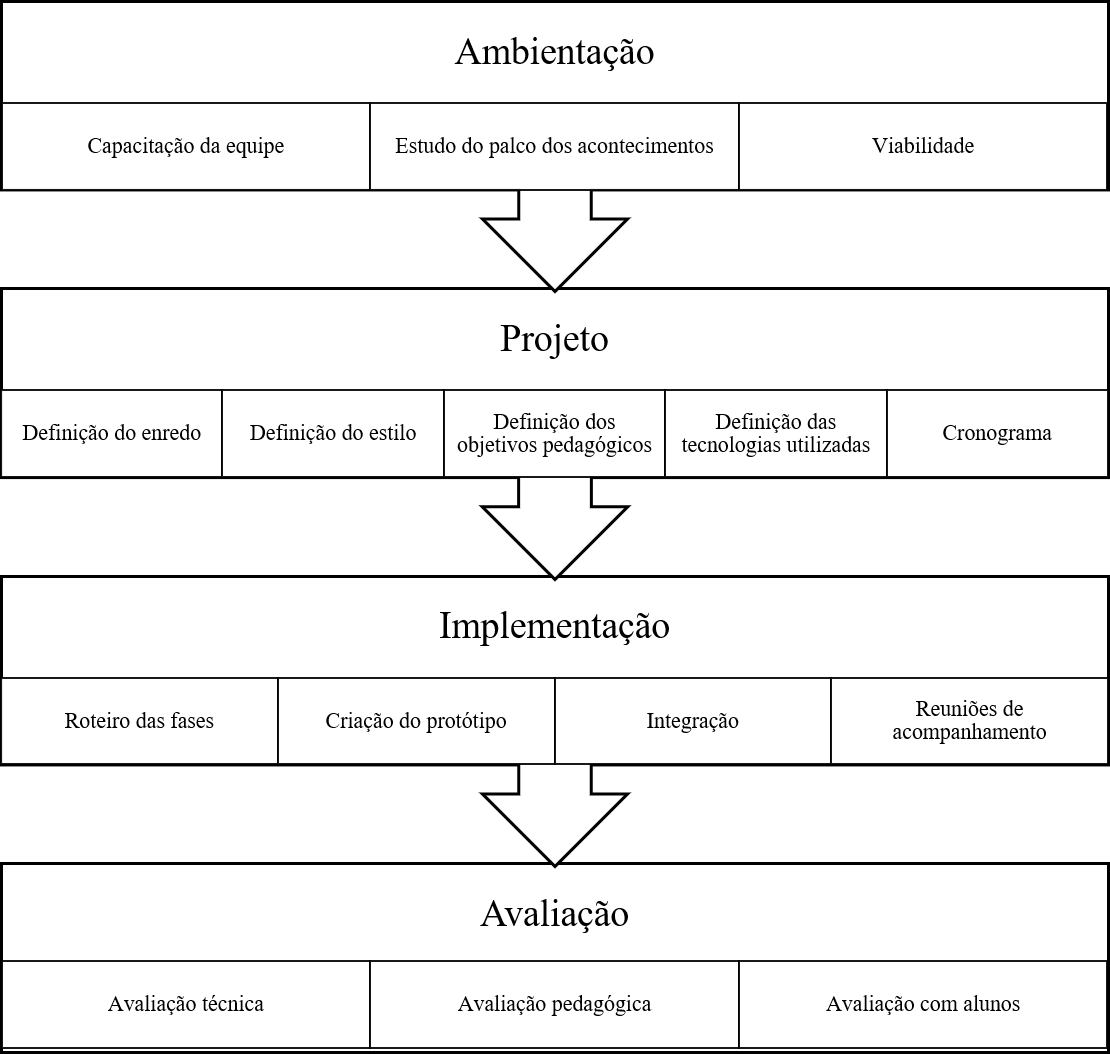
\includegraphics[width=0.73\textwidth]{figuras/framework_dev.PNG}
	\label{fig:framework_dev}
	{\fonte{O Autor (2018)}}
\end{figure}

O processo de desenvolvimento apresentado na figura \ref{fig:framework_dev}, é composto por quatro etapas (retângulos grandes) e quinze práticas (retângulos pequenos). Os tópicos abaixo apresentam cada uma das etapas adotadas neste processo, explicando as respectivas práticas.

\begin{itemize}

\item \textbf{Ambientação:} É aqui que a equipe do projeto realiza um \textit{estudo sobre o palco dos acontecimentos} que irão compor o jogo digital, identificando eventos-chave que podem \textit{viabilizar} a implementação do jogo ou colaborar para ela. Além disso, nesta etapa a equipe do projeto começa a se \textit{capacitar} continuamente para implementá-lo, por meio de cursos sobre ferramentas, métodos e tecnologias a serem empregadas.

\item \textbf{Projeto:} Inicia com a definição do \textit{enredo do jogo educativo}, bem como a \textit{definição do estilo} deste (plataforma \textit{2D}, \textit{RPG}, \textit{FPS} e etc). Posteriormente, são definidos os \textit{objetivos pedagógicos} do jogo, ou seja, quais conteúdos serão repassados durante o jogo e como isso vai acontecer, por exemplo, por meio de tirinhas \cite{bib:bb2016}, de bônus de informação \cite{bib:teixeira2016} e etc. Após isso, a equipe \textit{define as tecnologias} a serem empregadas (\textit{game engine}, plataformas alvo, editores de imagem e etc) e o \textit{cronograma de atividades} do projeto. Todas estas etapas são integradas no \textit{GDD (Game Design Document)}, que é um documento em que se enumera e especifica todos os aspectos quantitativos e qualitativos de um jogo, tais como: mecânica (sistema de regras), \textit{level design} (cenários), \textit{character design} (personagens), programação (interatividade) e etc.

\item \textbf{Implementação:} Com base no enredo definido na etapa anterior, são elaborados os \textit{roteiros dos levels} e os membros da equipe começam a trabalhar na \textit{criação do protótipo} do jogo. Em geral, uma equipe de desenvolvimento de jogos é composta por programadores e artistas, que trabalham em conjunto para a criação dos \textit{levels}, os artistas trabalham na criação dos objetos e cenários e os programadores na codificação, com base no que fora definido no roteiro. Finalizado o protótipo, a equipe do projeto realiza a integração dos \textit{levels}, criando uma versão executável do jogo. Durante esta etapa, ocorrem várias \textit{reuniões de acompanhamento}, com o propósito de verificar o alinhamento aos objetivos gerais do projeto.

\item \textbf{Avaliação:} Foi extraída da metodologia proposta por \citeonline{bib:guterres2017}. Dividida em três: \textit{avaliação técnica}, que a equipe do projeto realiza, geralmente para a verificação de erros e inconsistências durante a jogatina; \textit{avaliação pedagógica}, que objetiva checar a adequação do jogo educativo ao seu objetivo pedagógico, ou seja, fazer a verificação da adequação pedagógica do jogo às características do público alvo; e finalizando com a \textit{avaliação com alunos}, que é a realização de coleta de dados sobre o uso do jogo pelos alunos (questionários, entrevistas e etc), analisando as dificuldades encontradas no uso deste, avaliando a sua eficácia.

\end{itemize}

\section{Especificações Técnicas}
\label{sec:especificacoes}

Nas seções abaixo são apresentadas as especificações técnicas, tanto dos requisitos de hardware do público alvo do jogo (usuários), como do computador que foi utilizado pelo autor deste trabalho para desenvolver o game.

\newpage

\addtocontents{toc}{\protect\setcounter{tocdepth}{1}}
\subsection{Requisitos de Hardware Alvo}

A primeira versão completa do jogo foi gerada para a plataforma \textit{mobile}, especificamente para o sistema operacional \textit{Android}. Após uma série de testes, a equipe definiu os requisitos mínimos necessários para um \textit{smartphone} executar o game, que estão listados na tabela \ref{tab:reqmin} (lado esquerdo). Pensando em executar o jogo no sistema operacional \textit{Windows}, a equipe definiu também os requisitos mínimos para um \textit{Personal Computer (PC)} -- computador pessoal \textit{(desktop)} executar o game, conforme a tabela \ref{tab:reqmin} (lado direito).

\begin{table}[htb]
	\IBGEtab{%
		\caption{Requisitos mínimos de hardware alvo (\textit{smartphone} e \textit{PC})}%
		\label{tab:reqmin}
	}{%
		\begin{tabular}{lll}
			\toprule
			\textbf{Sistema Operacional} & \textit{Android} 5.0 \textit{`Lollipop' API} 21 & \textit{Microsoft Windows 7 32 bits} \\
			\midrule
			\textbf{Processador} & 1 Núcleo de 1GHz & 2 Núcleos de 2GHz \\
			\midrule
			\textbf{Memória RAM} & 1GB & 4GB \\
			\midrule
			\textbf{Vídeo} & 128MB & 512MB \\
			\midrule
			\textbf{Armazenamento} & 8GB & 250GB \\
			\midrule
			\textbf{Entrada} & Tela \textit{touch} & teclado e \textit{mouse} \\
			\midrule
			\textbf{Saída} & Dispositivo de audio & Dispositivo de audio \\
			\bottomrule
		\end{tabular}%
	}{%
		\fonte{O Autor (2018)}
	}
\end{table}

\addtocontents{toc}{\protect\setcounter{tocdepth}{1}}
\subsection{Ambiente de Desenvolvimento}

A equipe do projeto possui um espaço físico com um único computador de mesa, o que acaba fazendo com que os membros usem seus computadores pessoais para a realização de suas designações. O autor deste trabalho usou o seu \textit{notebook} pessoal para o desenvolvimento desta pesquisa. A tabela \ref{tab:reqdev} mostra as configurações deste \textit{notebook}.

\begin{table}[htb]
	\IBGEtab{%
		\caption{Ambiente de desenvolvimento utilizado}%
		\label{tab:reqdev}
	}{%
		\begin{tabular}{ll}
			\toprule
			\textbf{Sistema Operacional} & \textit{Windows 10 Home Single Language 64-bits} \\
			\midrule
			\textbf{Processador} & \textit{Intel(R) Core(TM) i7-4510U CPU @ 3.1GHz} \\
			\midrule
			\textbf{Memória RAM} & 16GB \\
			\midrule
			\textbf{Vídeo} & \textit{AMD Radeon R7 M265 2GB} \\
			\midrule
			\textbf{Armazenamento} & 1TB \\
			\midrule
			\textbf{Entrada} & \textit{Display LCD 15.6 pol. $1920\times1080$ (32 bit) (60Hz)} com \textit{touch} \\
			\midrule
			\textbf{Saída} & Alto falantes \textit{(Realtek High Definition Audio)} \\
			\bottomrule
		\end{tabular}%
	}{%
		\fonte{O Autor (2018)}
	}
\end{table}
